\chapter{Backup}
\label{chap:Backup}

\section{Dilepton Plots with \mediumPP\ Electrons}
\graphicspath{{Chapters/ObjEventSelection/Figures/}}

\begin{figure}[h]
\centering
	\subfigure[7~\tev]{
            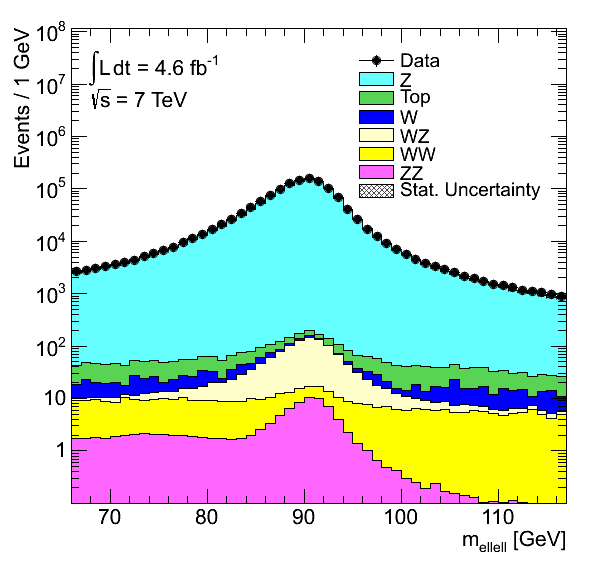
\includegraphics[width=0.47\textwidth]{Dilepton7TeV/CeECeE_pt20MediumPP_Z_m}
        }
	\subfigure[8~\tev]{
            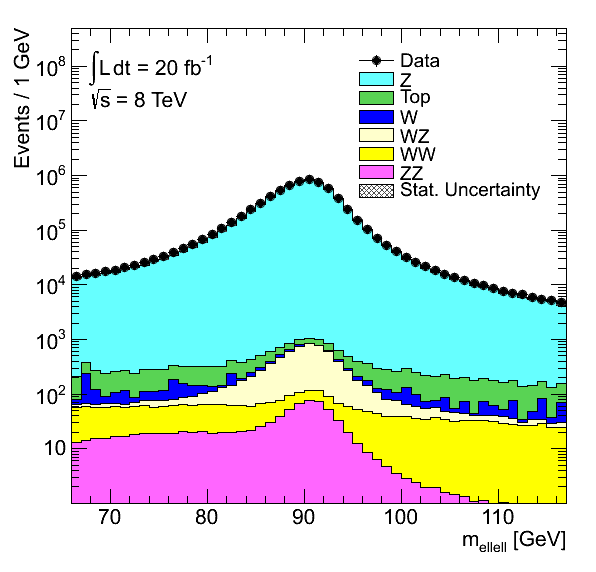
\includegraphics[width=0.47\textwidth]{Dilepton8TeV/CeECeE_pt20MediumPP_Z_m}
        }
	\subfigure[7~\tev]{
            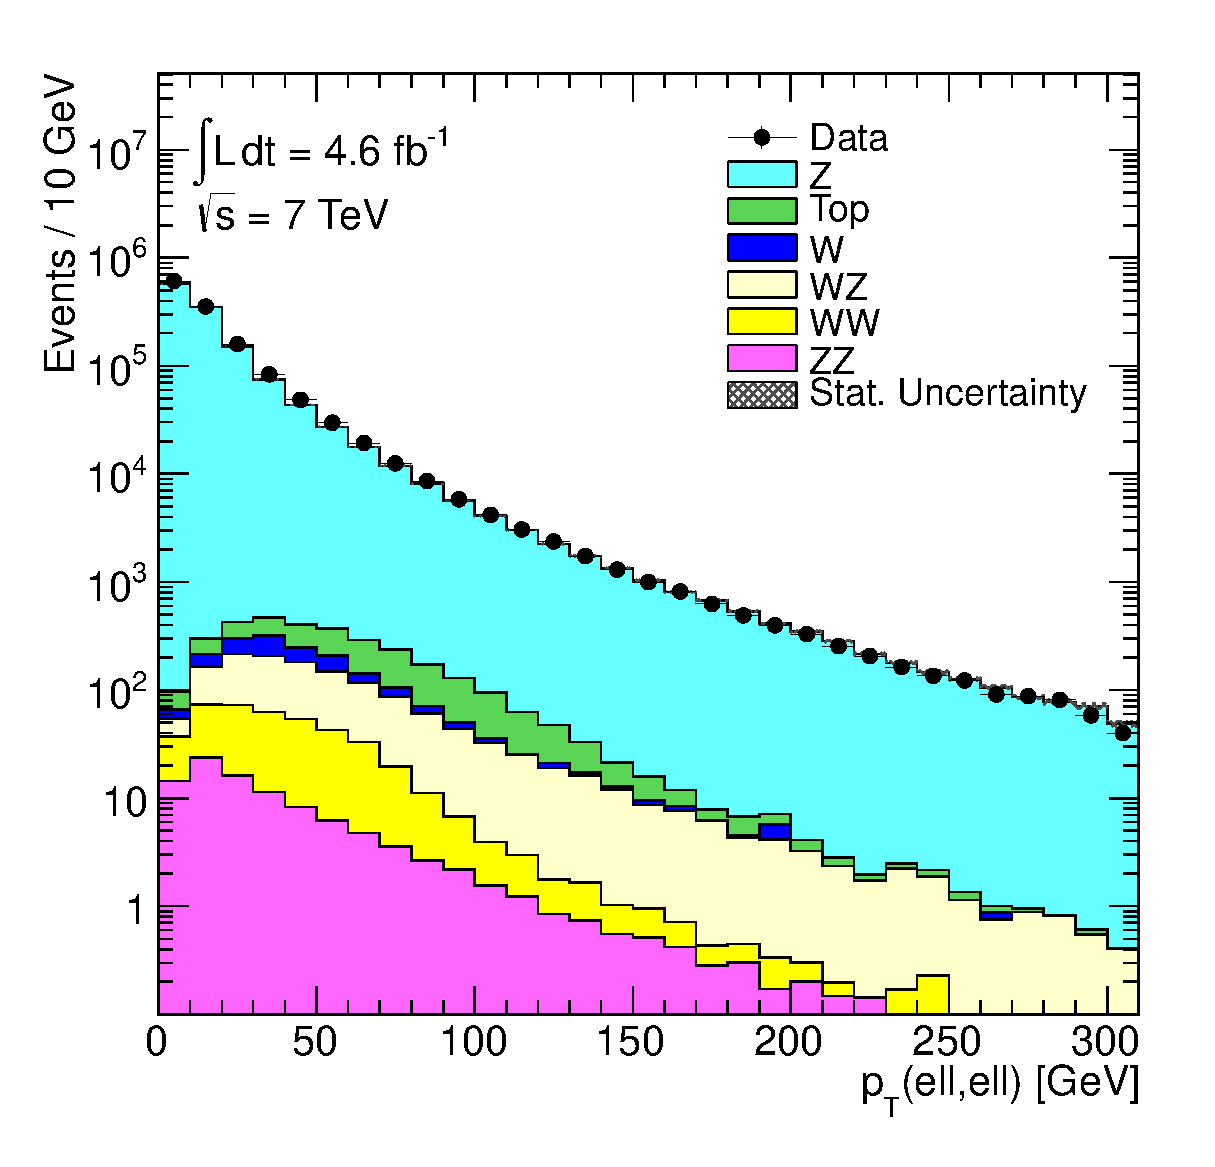
\includegraphics[width=0.47\textwidth]{Dilepton7TeV/CeECeE_pt20MediumPP_Z_pt}
        }
	\subfigure[8~\tev]{
            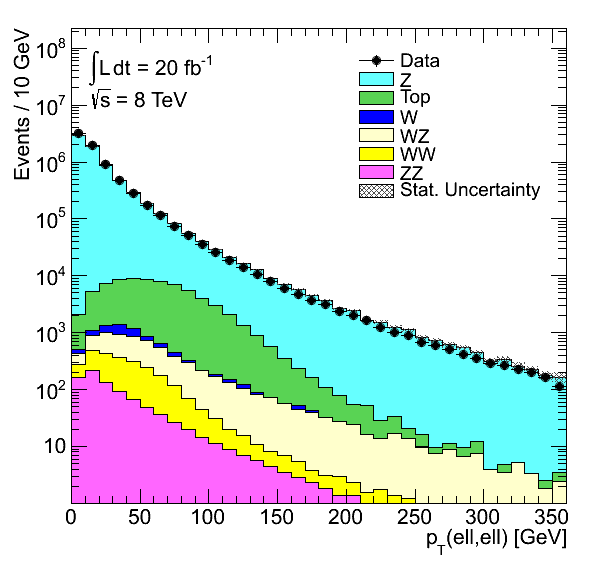
\includegraphics[width=0.47\textwidth]{Dilepton8TeV/CeECeE_pt20MediumPP_Z_pt}
        }
    \caption[Dilepton invariant mass and transverse momentum in the 7~\tev\
    data. ]
    {Kinematic distributions for
    \dielectron\ pairs, for the 7~\tev\ and the 8~\tev\ data respectively, in events containing a pair of
    \ossf\ electrons with the electron selection tightened to require both
    electrons satisfy the \mediumPP\ requirements and have \ptgt{20}. 
    }
\label{fig:dilep-mass-pt-seven}
\end{figure}

\begin{figure}[h]
\centering
\vspace{-5mm}
	\subfigure[7~\tev]{
            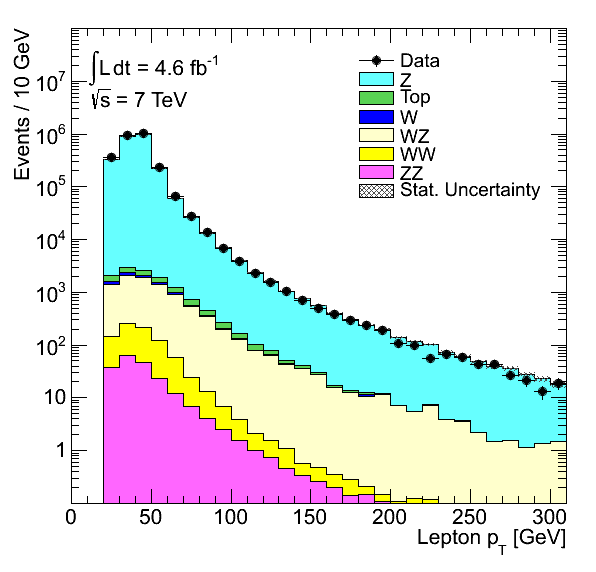
\includegraphics[width=0.47\textwidth]{Dilepton7TeV/CeECeE_pt20MediumPP_lep_pt}
        }
	\subfigure[8~\tev]{
            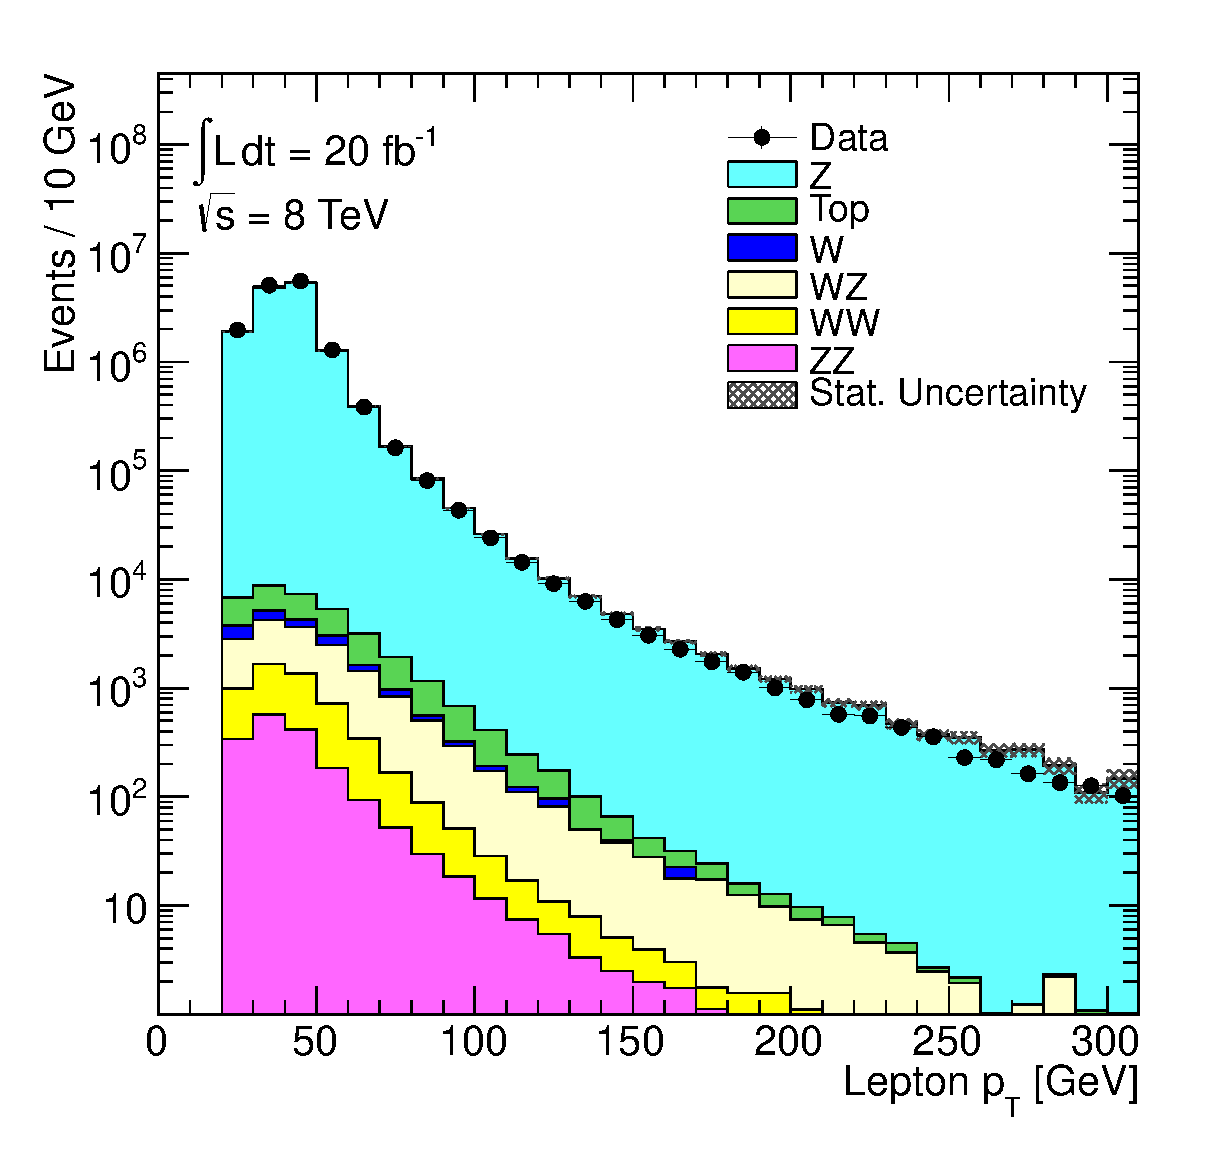
\includegraphics[width=0.47\textwidth]{Dilepton8TeV/CeECeE_pt20MediumPP_lep_pt}
        }
	\subfigure[7~\tev]{
            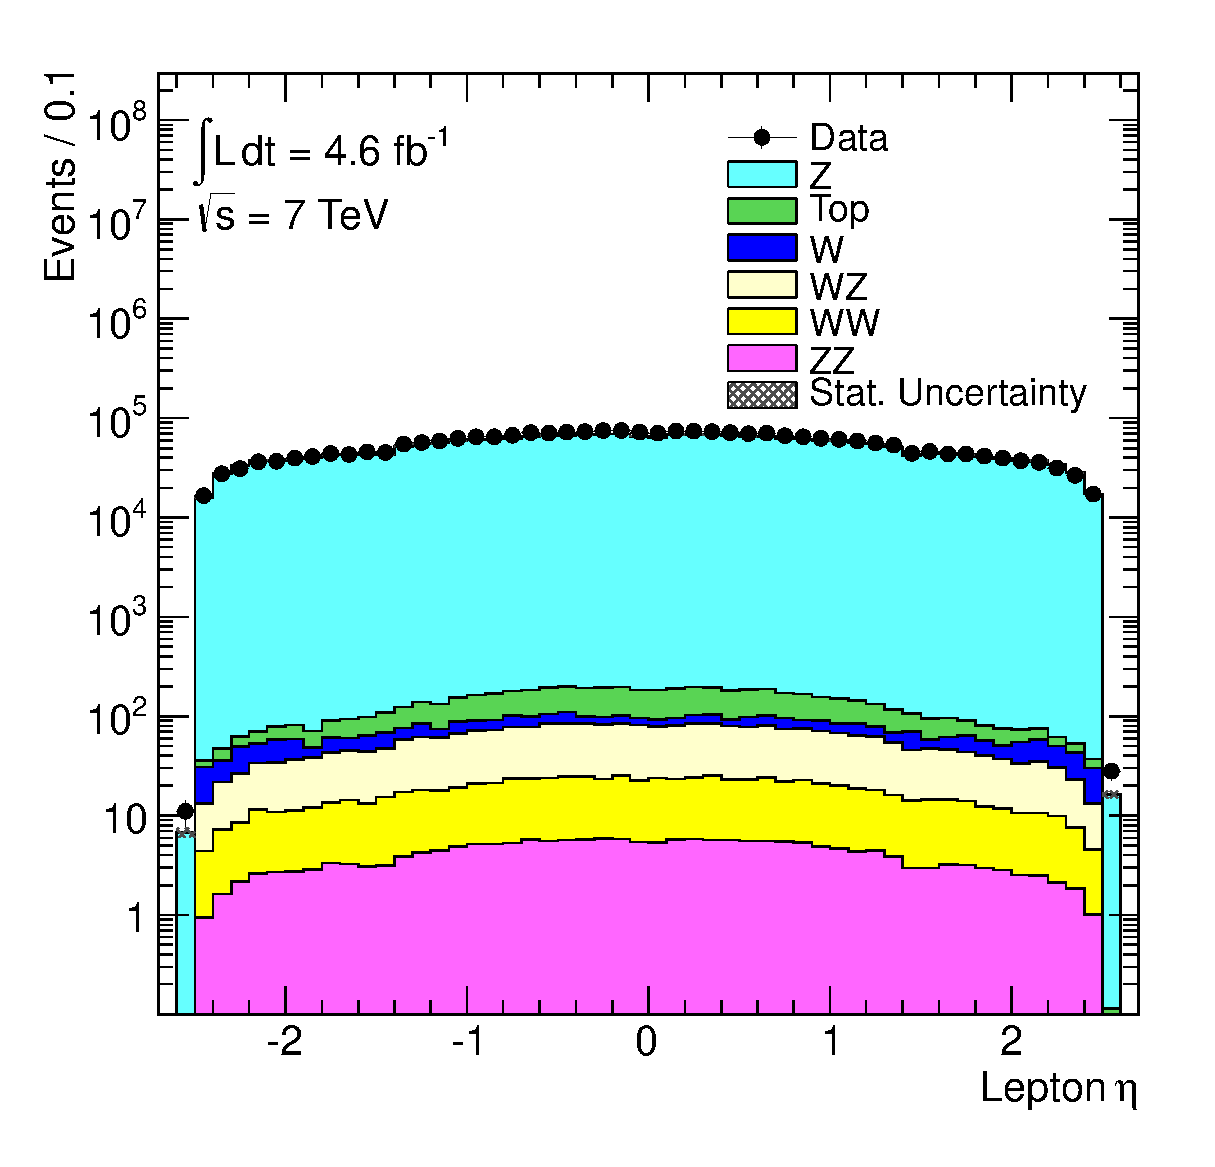
\includegraphics[width=0.47\textwidth]{Dilepton7TeV/CeECeE_pt20MediumPP_lep_eta}
        }
	\subfigure[8~\tev]{
            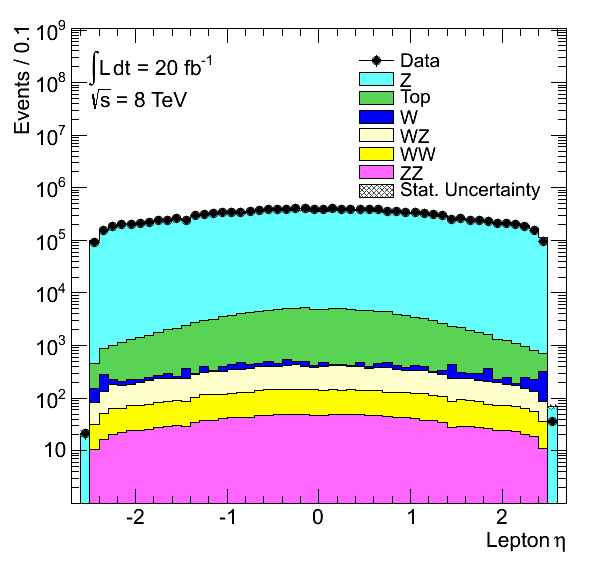
\includegraphics[width=0.47\textwidth]{Dilepton8TeV/CeECeE_pt20MediumPP_lep_eta}
        }
	\subfigure[7~\tev]{
            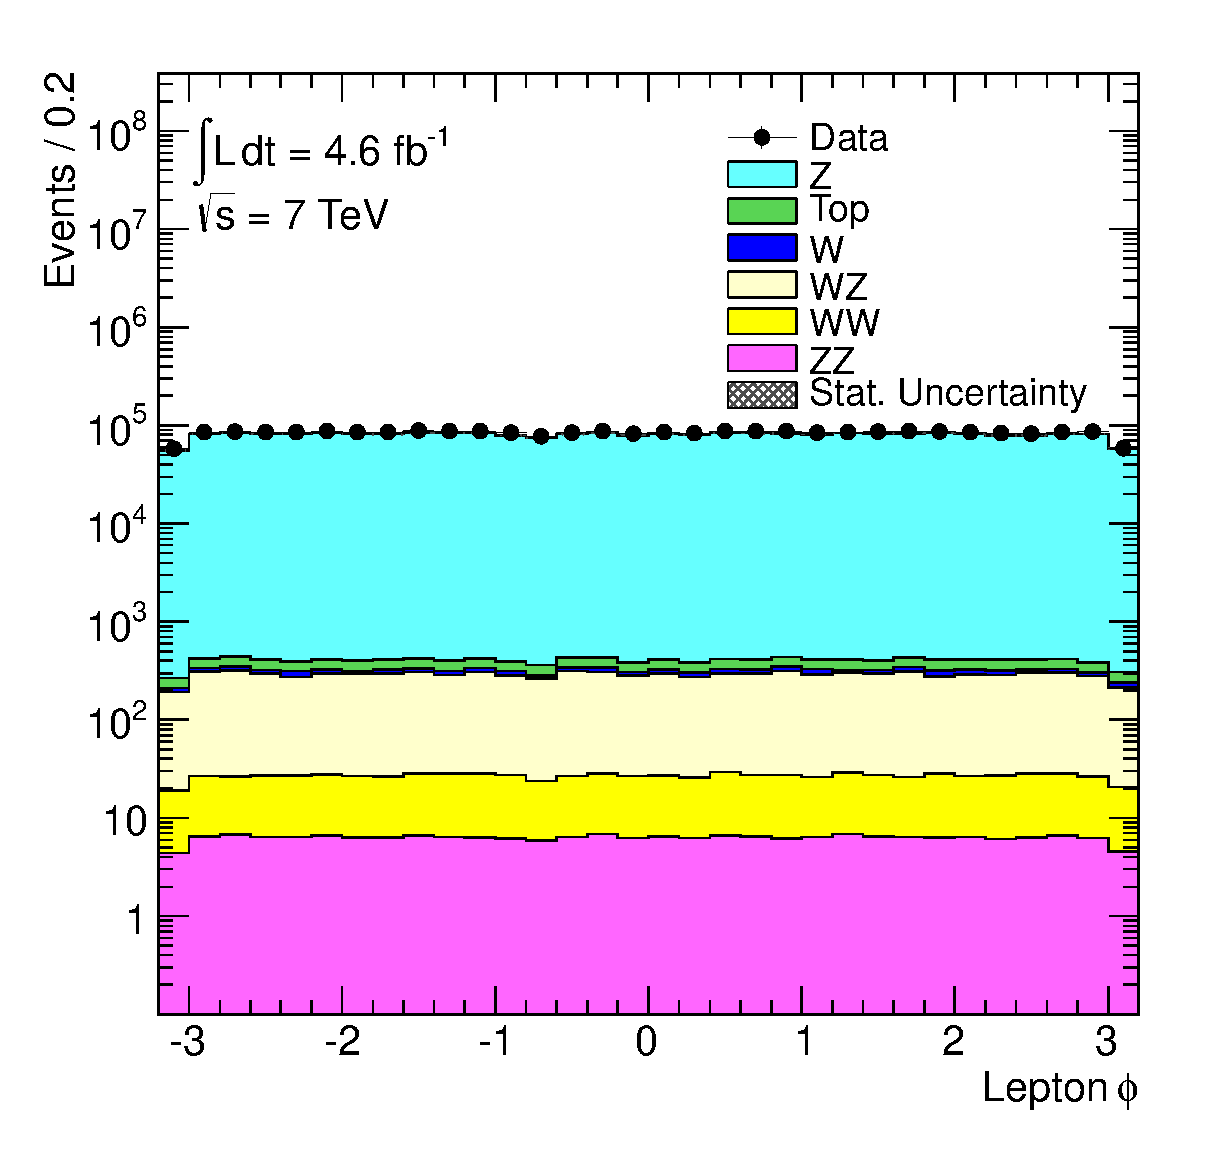
\includegraphics[width=0.47\textwidth]{Dilepton7TeV/CeECeE_pt20MediumPP_lep_phi}
        }
	\subfigure[8~\tev]{
            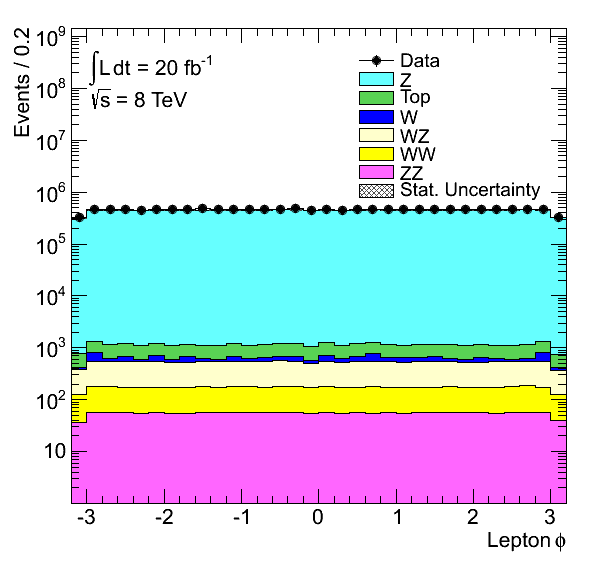
\includegraphics[width=0.47\textwidth]{Dilepton8TeV/CeECeE_pt20MediumPP_lep_phi}
        }
    \caption[Lepton kinematic distributions for \dilep\ events in the 7~\tev\
    data. ]
    {\small Kinematic distributions for
    electron  in events containing a pair of
    \ossf\ electrons, with the electron selection tightened to require both
    electrons satisfy the \mediumPP\ requirements and have \ptgt{20}, for the 7~\tev\ and the 8~\tev\ data. }
\label{fig:dilep-lepkin-seven}
\end{figure}

\graphicspath{{Chapters/Backup/Figures/}}

\begin{figure}[h]
\centering
	\subfigure[7~\tev]{
            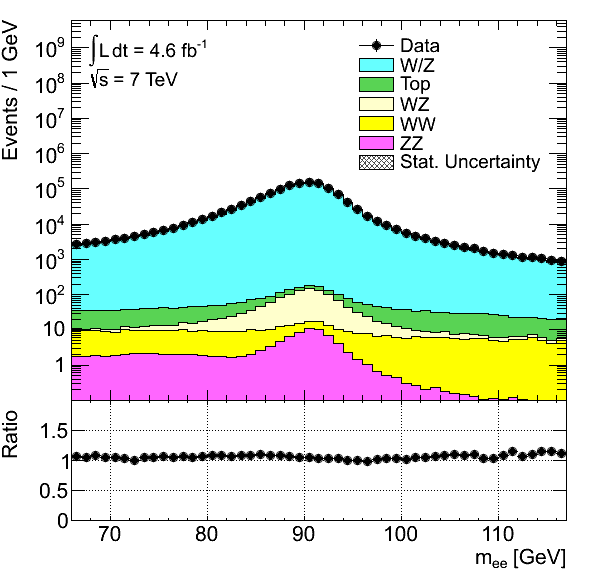
\includegraphics[width=0.47\textwidth]{Dilepton7TeVRatio/CeECeE_pt20MediumPP_Z_m}
        }
	\subfigure[8~\tev]{
            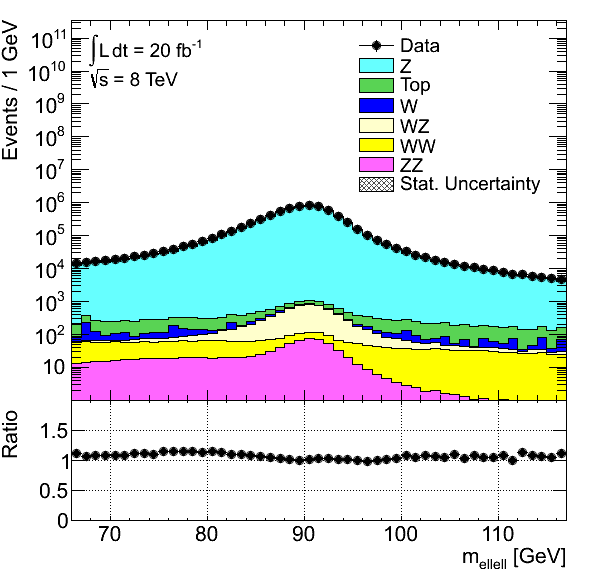
\includegraphics[width=0.47\textwidth]{Dilepton8TeVRatio/CeECeE_pt20MediumPP_Z_m}
        }
	\subfigure[7~\tev]{
            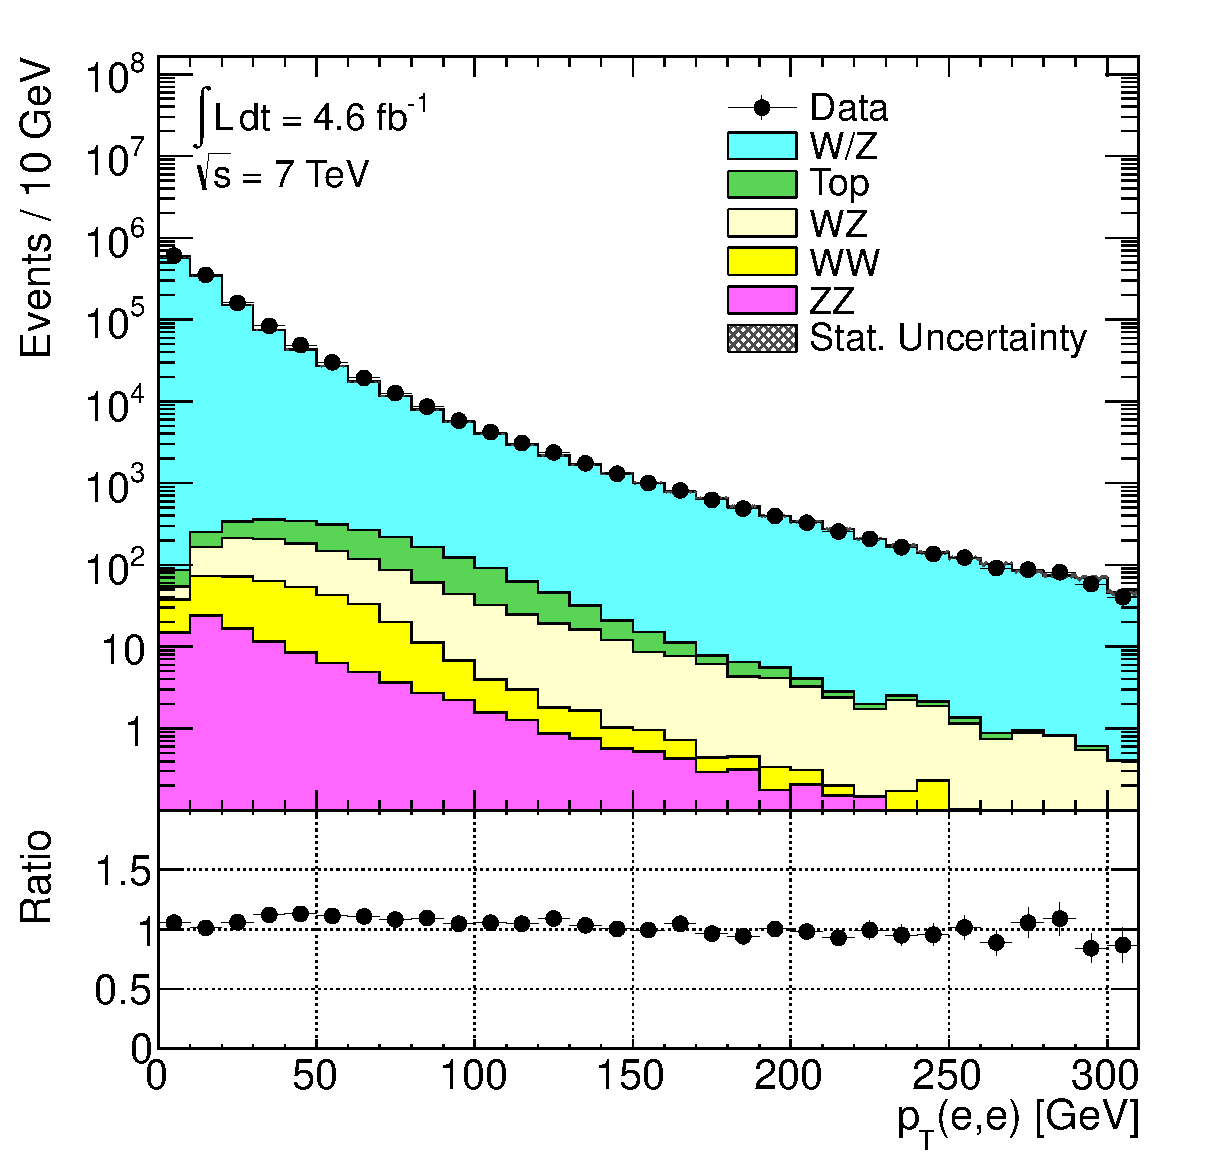
\includegraphics[width=0.47\textwidth]{Dilepton7TeVRatio/CeECeE_pt20MediumPP_Z_pt}
        }
	\subfigure[8~\tev]{
            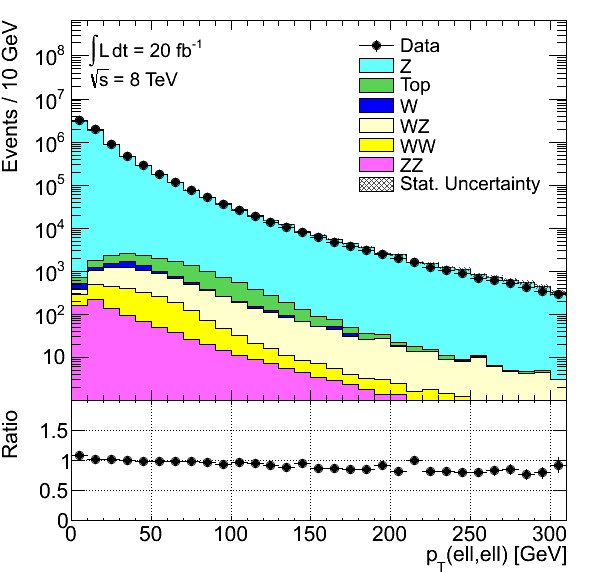
\includegraphics[width=0.47\textwidth]{Dilepton8TeVRatio/CeECeE_pt20MediumPP_Z_pt}
        }
    \caption[Dilepton invariant mass and transverse momentum in the 7~\tev\
    data. ]
    {Kinematic distributions for
    \dielectron\ pairs, for the 7~\tev\ and the 8~\tev\ data respectively, in events containing a pair of
    \ossf\ electrons with the electron selection tightened to require both
    electrons satisfy the \mediumPP\ requirements and have \ptgt{20}. 
    }
\label{fig:dilep-mass-pt-seven}
\end{figure}

\begin{figure}[h]
\centering
\vspace{-5mm}
	\subfigure[7~\tev]{
            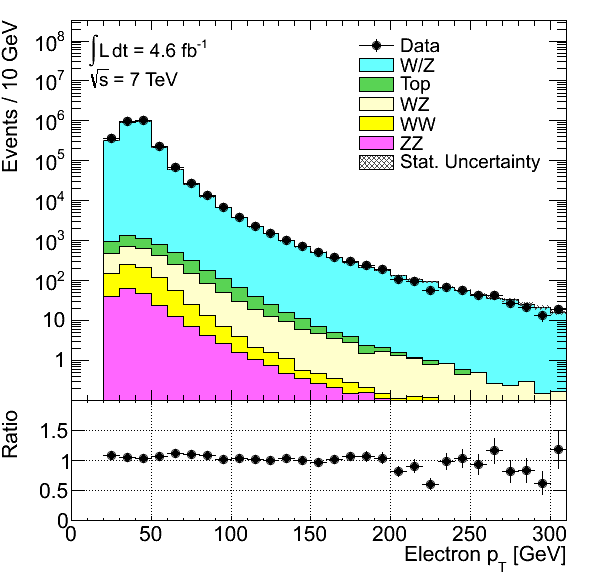
\includegraphics[width=0.47\textwidth]{Dilepton7TeVRatio/CeECeE_pt20MediumPP_lep_pt}
        }
	\subfigure[8~\tev]{
            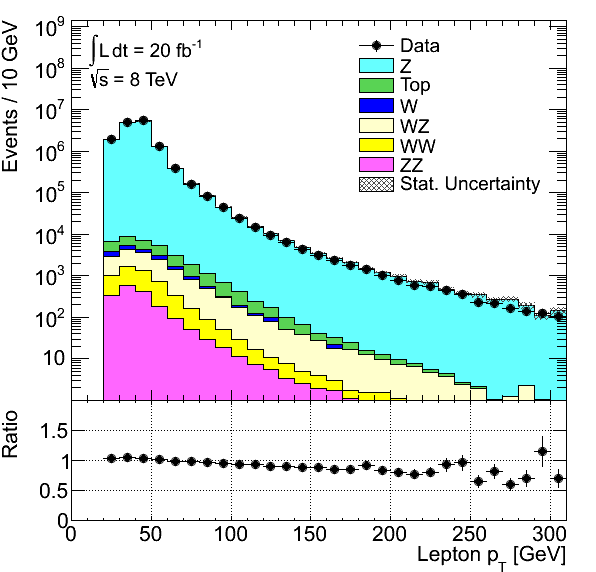
\includegraphics[width=0.47\textwidth]{Dilepton8TeVRatio/CeECeE_pt20MediumPP_lep_pt}
        }
	\subfigure[7~\tev]{
            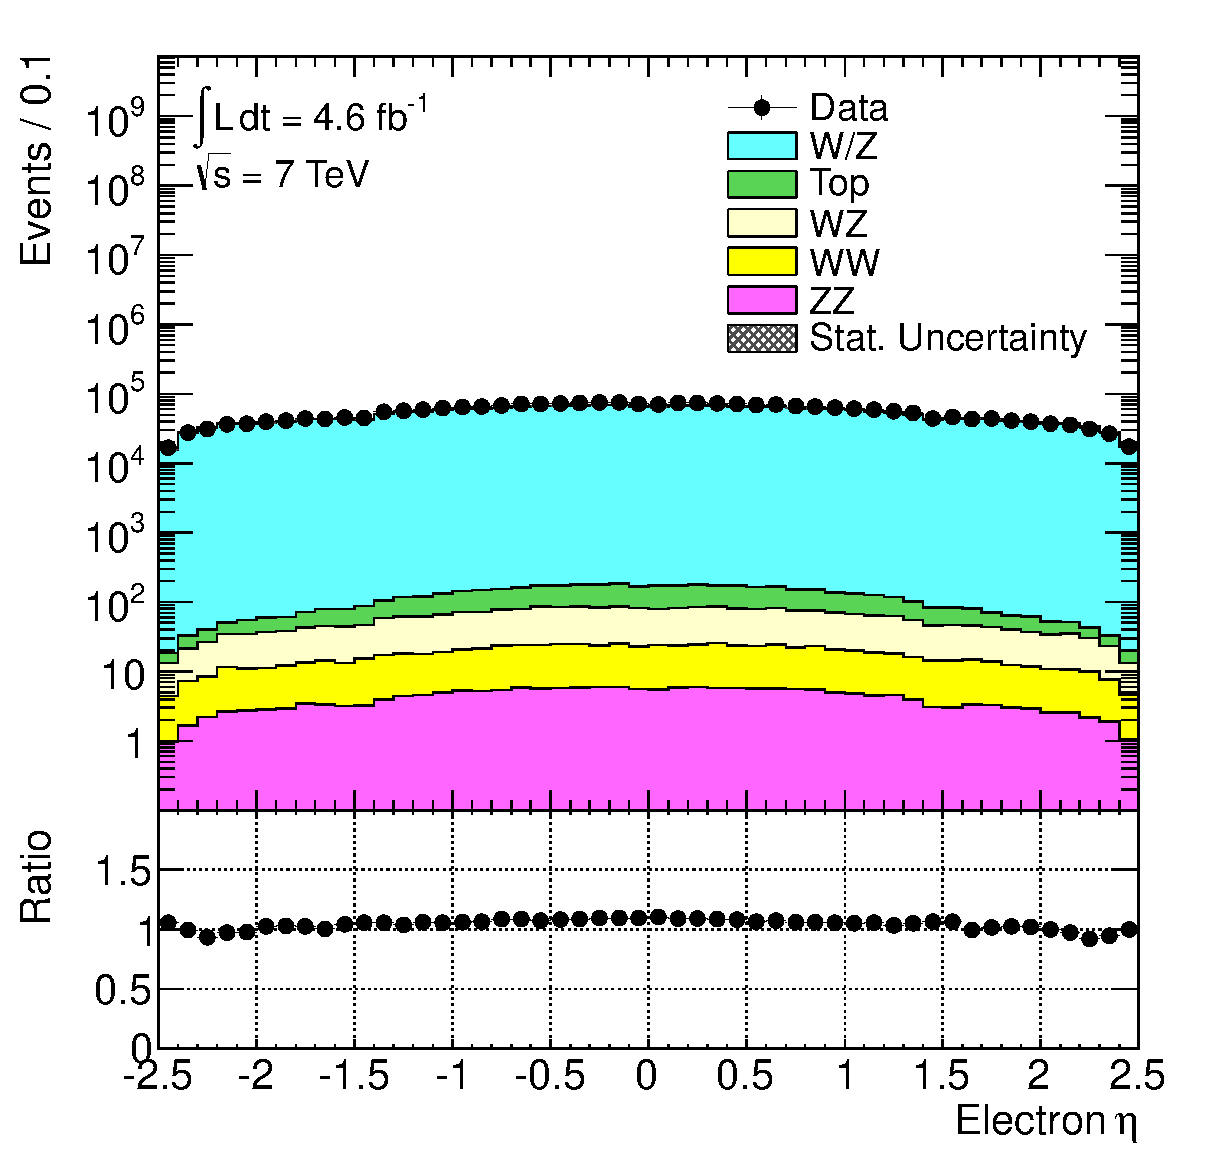
\includegraphics[width=0.47\textwidth]{Dilepton7TeVRatio/CeECeE_pt20MediumPP_lep_eta}
        }
	\subfigure[8~\tev]{
            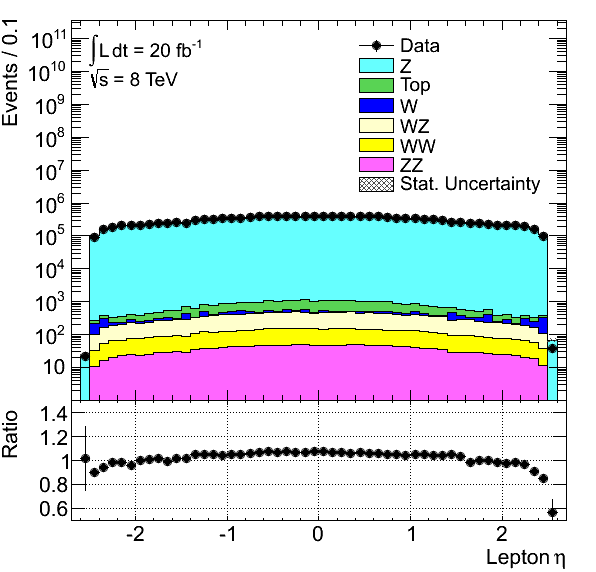
\includegraphics[width=0.47\textwidth]{Dilepton8TeVRatio/CeECeE_pt20MediumPP_lep_eta}
        }
	\subfigure[7~\tev]{
            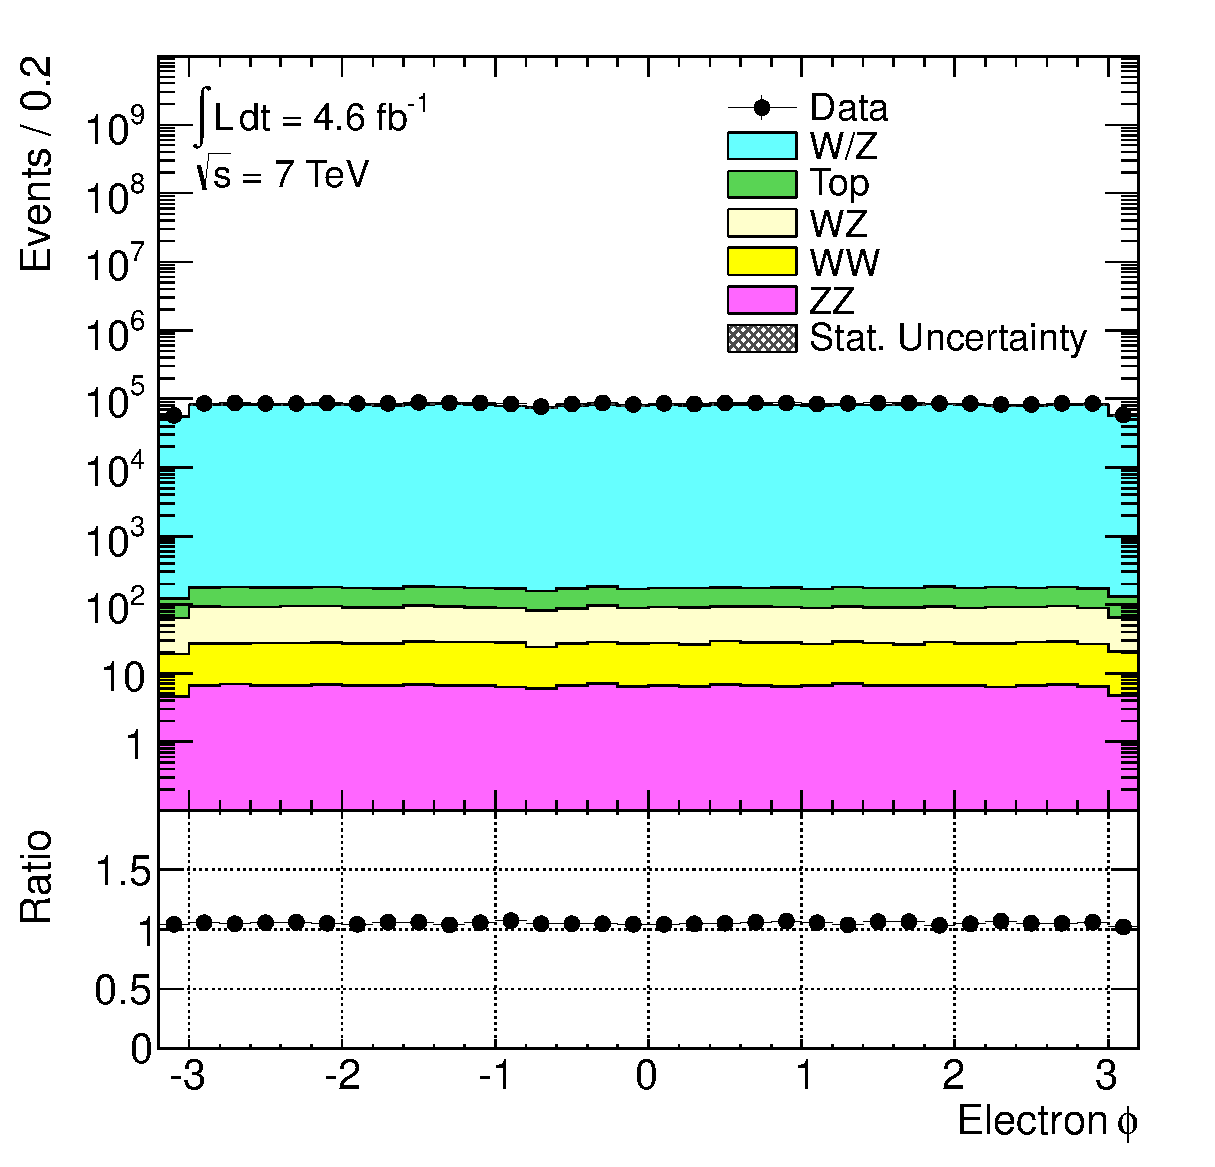
\includegraphics[width=0.47\textwidth]{Dilepton7TeVRatio/CeECeE_pt20MediumPP_lep_phi}
        }
	\subfigure[8~\tev]{
            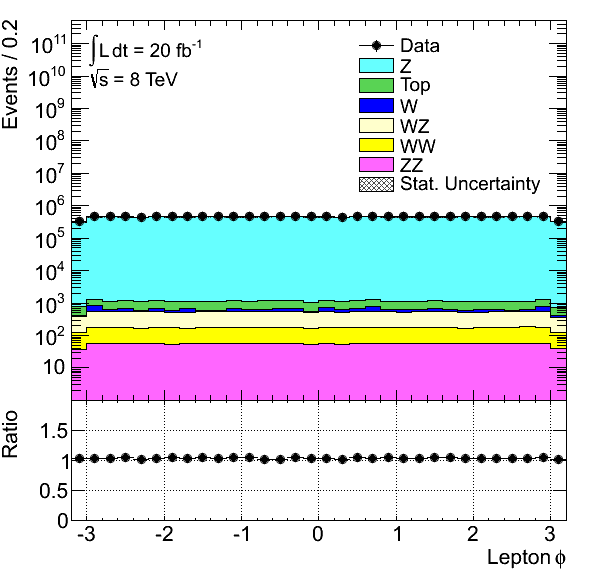
\includegraphics[width=0.47\textwidth]{Dilepton8TeVRatio/CeECeE_pt20MediumPP_lep_phi}
        }
    \caption[Lepton kinematic distributions for \dilep\ events in the 7~\tev\
    data. ]
    {\small Kinematic distributions for
    electron  in events containing a pair of
    \ossf\ electrons, with the electron selection tightened to require both
    electrons satisfy the \mediumPP\ requirements and have \ptgt{20}, for the 7~\tev\ and the 8~\tev\ data. }
\label{fig:dilep-lepkin-seven}
\end{figure}
